\chapter{Scelta tecnologica}
\label{chap:scelta}
\nocite{rest}

In questo capitolo illustreremo i meccanismi di base della nostra applicazione e modelleremo i nostri dati, per poi continuare scrivendo i test che valideranno il comportamento della nostra applicazione e descriveremo come è organizzato il nostro codice.


Per sviluppare la nostra applicazione abbiamo utilizzato lo stack MEAN\index{MEAN} che può essere sintetizzato come segue
\begin{itemize}
\item M = MongoDB/Mongoose.js: il popolare database, e l'elegante ODM per Node.js
\item E = Express.js: un framework web leggero
\item A = Angular.js: un framework per la creazione di single page application
\item N = Node.js: un interprete JavaScript costruito sul motore JavaScript V8 di Google Chrome orientato agli eventi che lo rende efficiente e leggero.
\end{itemize}
Lo stack MEAN è un sostituto dello stack LAMP\index{LAMP} (Linux, Apache, MySQL, PHP/Perl/Python/P…) molto popolare per la costruzione di applicazione web negli anni 90.

In questa tesi non descriveremo Angular perché verrà fatto nell'elaborato di Marco in cui descriverà il frontend. 
Andiamo quindi a costruire le REST API che non hanno una user interface, ma sono la nostra base per qualsiasi tipo di applicazione, come un sito web, un'app Android, iOS o Ubuntu Touch.

\section{JSON}
\nocite{ajax}
JSON è un formato di dati molto leggere basato su un sottoinsieme della sintassi JavaScript, cioè \emph{array literal} e \emph{object literal}, proposto da Douglas Crockford come formato per i servizi web in sostituzione al verboso XML\index{XML}.
Dato l'utilizzo della sintassi Javascript, le definizioni JSON\index{JSON} possono essere incluse all'interno dei file JavaScript ed è possibile accedervi senza l'analisi aggiuntiva necessaria con i linguaggi basati su XML.
\subsection{Gli array literal}

Gli \emph{array literal} rappresentano il metodo più semplice per creare un Array in javaScript.
Infatti, basta elencare una lista di valori separati da una virgola all'interno delle parentesi quadre, per esempio:
\begin{lstlisting}[style=JavaScriptCode]
var users = ["Saverio", "Marco", "Francesco"];
\end{lstlisting}
Funzionalmente parlando è equivalente alla forma tradizionale:
\begin{lstlisting}[style=JavaScriptCode]
var users = new Array("Saverio", "Marco", "Francesco");
\end{lstlisting}
Entrambe le definizioni generano lo stesso risultato ed è possibile accedere ad ogni elemento dell'array utilizzando il relativo indice 
\begin{lstlisting}[style=JavaScriptCode]
console.log(users[0]); \\Saverio 
console.log(users[1]); \\Marco
console.log(users[2]); \\Francesco
\end{lstlisting}
Quando si parla di array in JavaScript è bene tenere in mente due cose.
La prima è che JavaScript non è tipizzato e quindi l'array può contenere tipi di dati completamente diversi.
La seconda è che nonostante entrambi i metodi per la creazione di un array siano leciti in JavaScript, soltanto gli array literal sono validi in JSON.
\subsection{Gli object literal}
Un object literal è definito tra parentesi graffe.
Al loro interno troviamo un numero qualsiasi di coppie chiave-valore, definite con una stringa, i due punti ed il valore.
Ogni coppia deve essere seguita da una virgola, eccetto l'ultima. 
Questo insieme di coppie chiave-valore rappresenta alla fine un oggetto.
Un esempio:
\begin{lstlisting}[style=JavaScriptCode]
var user = {
	"firstname": "Saverio",
	"permission": 0,
	"block": false
};
\end{lstlisting}
Il codice qui sopra genera un oggetto user con le proprietà firstname, permission e block. 
Per accedere alle proprietà dell'oggetto basta usare la notazione con il punto
\begin{lstlisting}[style=JavaScriptCode]
console.log(user.firstname); \\"Saverio"
console.log(user.permission); \\"0"
console.log(user.block); \\"false"
\end{lstlisting}
Lo stesso oggetto potrebbe essere creato utilizzando il costruttore \texttt{Object} di JavaScript
\begin{lstlisting}[style=JavaScriptCode]
var user = new object():
user.firstname = "Saverio";
user.permission = 0;
user.block = false;
\end{lstlisting}
Anche in questo caso, sebbene entrambi gli approcci siano validi in JavaScript, in JSON è valida solo la notazione object literal.
\subsection{La sintassi JSON}
La sintassi di JSON non è altro che il miscuglio di object literal ed array literal per memorizzare dati.
Quello che bisogna tener bene a mente è che JSON rappresenta solo dati.
Un esempio:
\begin{lstlisting}[style=JavaScriptCode]
[
	{
		"firstname": "Saverio",
		"permission": 0,
		"block": false
	},
	{
		"firstname": "Marco",
		"permission": 10,
		"block": false
	}
]
\end{lstlisting}
La prima cosa che salta all'occhio è che in questo documento non sono presenti variabili così come punti e virgola.
In questo modo quando si trasmette dei dati tramite HTTP ad un browser, il tutto avviene abbastanza velocemente grazie al numero ridotto di caratteri.

Oltre a questo, ci sono altri ovvi benefici dell'utilizzare JSON come formato dati per la comunicazione JavaScript: esso consente di non preoccuparsi della valutazione dei dati, e quindi, garantisce un accesso più veloce alle informazioni che essi contengono. 
Per un confronto dettagliato tra JSON e XML si rimanda alla bibliografia  \cite[pag. 251]{ajax}.
\section{REST}
REST sta per Representational State Transfer\cite{rest}. È una alternativa più semplice di SOAP e WSDL che sono protocolli basati su XML.

REST utilizza un modello client-server, dove il server è un server HTTP e il client invia richieste HTTP (GET, POST, PUT, DELETE), con un URL che al suo interno contiene i parametri codificati. L'URL describe l'oggetto e il server risponde, almeno nel nostro caso, con un codice e del JSON (JavaScript Object Notation).
In genere ci si aspetta che un server REST restituiasca un documento XML, sebbene nulla dell'architettura REST definisca il tipo di dati restituiti.
Un generico URL potrebbe restituire un'immagine, un documento HTML, un file CSV o qualunque altro tipo di dato.

Dato che utilizziamo lo stack MEAN, abbiamo scelto di utilizzare documenti JSON che risultano particolarmente adatti per la nostra applicazione, in cui tutti i nostri componenti sono in javascript e MongoDB interagisce perfettamente con questo formato. 
Faremo degli esempi più dettagliati più avanti quando definiremo i nostri Data Model.

L'acronimo CRUD è spesso utilizzato per descrivere le operazioni in un database. CRUD sta per CREATE, READ, UPDATE and DELETE. 
Queste operazioni possono essere facilmente mappate con i metodi HTTP, come segue:
\begin{itemize}
\item POST: Un client vuole inserire o creare un nuovo oggetto
\item GET: Un client vuole leggere un oggetto
\item PUT: Un client vuole aggiornare un oggetto
\item DELETE: Un client vuole eliminare un oggetto
\end{itemize}

Alcuni dei codici di risposta del protocollo HTTP che spesso vengono utilizzati insieme alle API REST sono i seguenti:
\begin{itemize}
\item 200 - “OK”
\item 201 - “Created” (Utilizzato con POST)
\item 400 - “Bad Request” (Ad esempio per l'assenza di parametri)
\item 401 - “Unauthorized” (Non ci poso i parametri per l'autenticazione)
\item 403 - “Forbidden” (L'utente è autenticato ma non ha i permessi)
\item 404 - “Not Found”
\end{itemize}
Una descrizione completa la si può trovare nel rispettivo RFC 2616\cite{RFC2616}

Lo sviluppo di API REST abilita lo sviluppo della fondamenta con il quale poi svilupperemo altre applicazioni. 
Come già detto precedentemente, queste applicazioni possono essere pensate per il web oppure specifiche di una determinata piattaforma.

Oggigiorno, ci sono molte aziende che sviluppano applicazione che non sono web, come Uber, WhatsApp, Postmates, and Wash.io. 
Le API REST permettono la facile implementazione su molte piattaforme che potranno essere sviluppate in un secondo momento, trasformando il progetto iniziale in un progetto indipendente dalla piattaforma utilizzata.

Possiamo iniziare a descrivere i dati che dobbiamo memorizzare:
\begin{itemize}
\item Dati degli utenti
\item Informazioni dei vari dispositivi
\item Dati dei beacon
\item GPIO(General Purpose Input Output)
\item Impostazioni del sistema
\end{itemize}
Diamo una sguardo alla prima collection:
\begin{lstlisting}[caption={User collection}, style=javaScriptCode]
{
    "_id": ObjectId("523b1153a2aa6a3233a913f8"),
    "username": "admin",
    "firstname": "Saverio",
    "lastname": "Tosi",
    "password": "123456",
    "permission": 0,
    "theme": "red",
    "block": false,
    "photo": "codificata in base 64"
}
\end{lstlisting}
Quando si parla di Database Relazionali si parla di Tabelle, righe e colonne.
In MongoDB, database non relazionale, c'è un collegamento con la maggior parte dei concetti dei Database Relazionali\index{Database}. Ad alto livello, MongoDB supporta uno o più database. 
Un database contiene una o più collezioni, che sono simili alle tabelle dei database relazionali. Le collezioni, a loro volta, contengono documenti. 
Ogni documento in una collezione è simile ad una riga di una tabella di un database relazionale. Con la differenza che un documento non segue uno schema specifico con colonne predefinite e con variabili semplici. 
Ogni documento consiste in una o più coppie chiave-valore dove il contenuto può essere o una variabile semplice oppure qualcosa di più complicato come un array.

Il documento JSON rappresenta un utente del nostro sistema. Lo scopo di ogni singolo campo è abbastanza intuitivo. Il campo più importante è \texttt{\_id}. 
In MongoDB, questo campo rappresenta la chiave primaria, se si salva un documento senza questo campo, esso verrà creato direttamente da MongoDB.

\begin{lstlisting}[caption={Beacon collection}, style=javaScriptCode]
{
    "_id": ObjectId("523b1153a2aa6a3233a913f8"),
    "uuid": "ACFD065E-C3C0-11E3-9BBE-1A514932AC01",
    "major": "0",
    "minor": "0",
    "state": "1"
}
\end{lstlisting}

Il documento che descrive i beacon conterrà soltanto 4 campi:
i primi tre sono quelli descritti nel capitolo precedente e rappresentano il payload del beacon; l'ultimo rappresenta lo stato del beacon, ovvero se esso è stato solo segnalato, se è stato registrato o se è stato eliminato e non deve essere più segnalato dagli utenti

\begin{lstlisting}[caption={Device collection}, style=javaScriptCode]
{
    "_id": ObjectId("523b1153a2aa6a3233a913f8"),
    "type": "Lampada",
    "io": "output",
    "permission": "0",
    "name": "Lampada Saverio",
    "description": "Lampada verde sulla scrivania",
    "automatic": false,
    "_GPIO": id_GPIO.
    "_Beacon": id_beacon,
    "properties": {}
}
\end{lstlisting}

Il documento che descrive il device memorizza: il tipo, se è di output o di input; il livello dei permessi; se deve essere comandato in maniera automatica; un riferimento al GPIO ed un riferimento al beacon associato. 
I permessi vanno da 0 a 10.
0 identifica l'admin, più è alto il valore di permission, più utenti potranno accedere al dispositivo.
In altre parole, un utente può accedere ad un dispositivo se e solo se il numero che identifica i permessi dell'utente(sempre da 0 a 10) è compreso tra 0 e il valore di permission del device  

\begin{lstlisting}[caption={GPIO collection}, style=javaScriptCode]
{
    "_id": ObjectId("523b1153a2aa6a3233a913f8"),
    "type": "output",
    "GPIO": 3,
    "_Device": id_device,
    "value": true
}
\end{lstlisting}

Un GPIO avrà soltanto le seguenti informazioni: il tipo, output o input; GPIO, che identifica il piedino nel raspberry; \_Device, un riferimento al dispositivo associato; value, che rappresenta il valore attuale del GPIO.

section

\section{Documentazione}
Una parte fondamentale della progettazione di API REST è la documentazione.
Per questa funzione abbiamo utilizzato i tool messi a disposizione da swagger\cite{swagger}\index{Swagger}.
\begin{figure}[htbp]
\centering
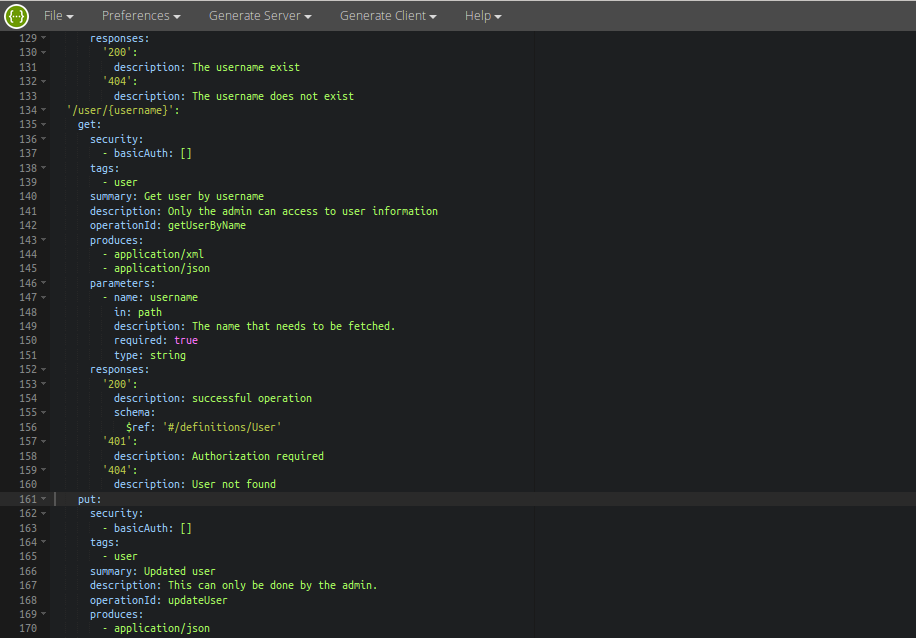
\includegraphics[scale=0.45]{Immagini/swagger-editor.png}
\caption{Swagger editor} 
\end{figure}\\

L'editor permette di descrivere le proprie API tramite un linguaggio chiamato YAML\index{YAML}
che rende la scrittura della documentazione semplice e veloce.
Quello che si ottiene è una documentazione interattiva, con la quale è anche possibili testare le API. 
\begin{figure}[htbp]
\centering
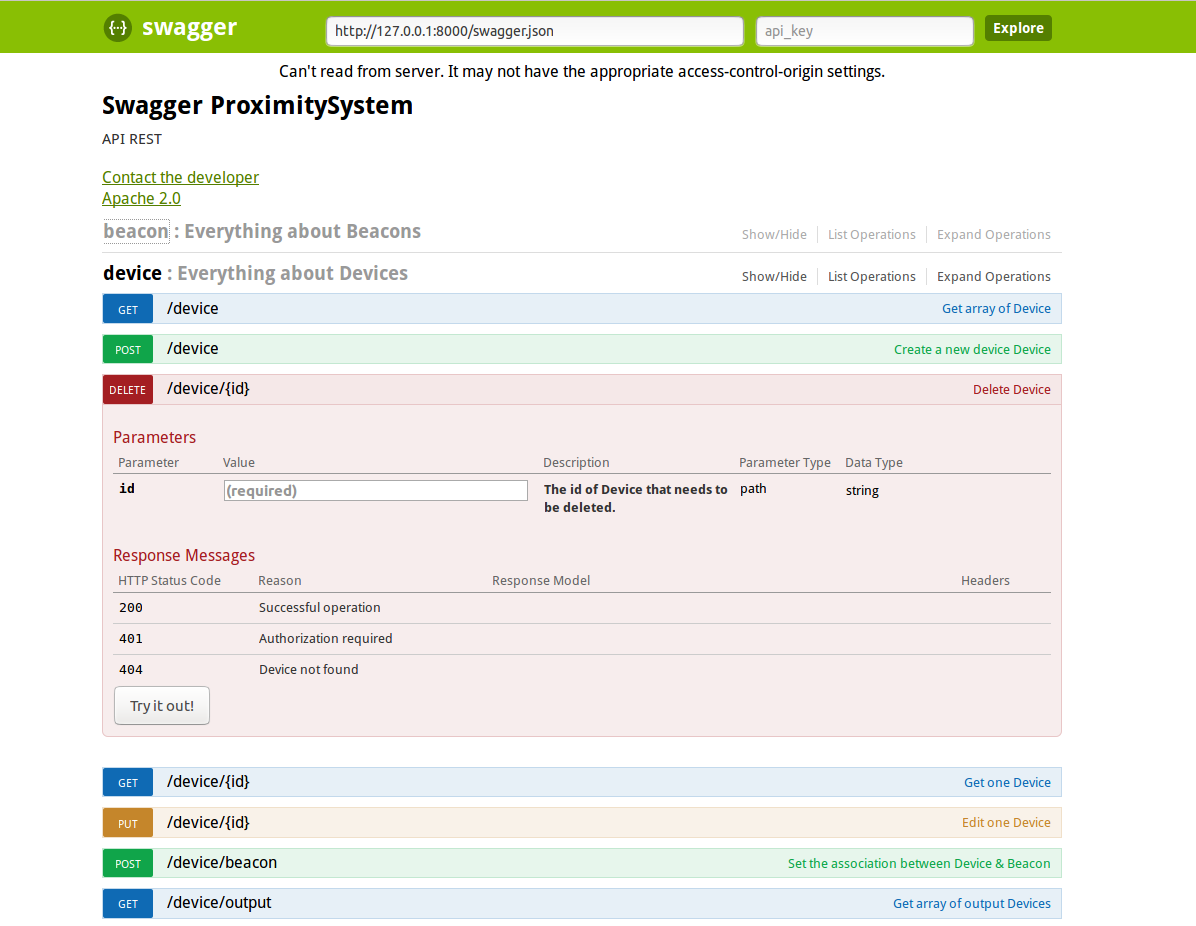
\includegraphics[scale=0.333]{Immagini/swagger-ui.png}
\caption{Swagger ui} 
\end{figure}

\newpage
\section{NodeJS}
Node.js\cite{node} è un interprete javascript per applicazioni di rete lato server. 
È disponibile per diverse piattaforme, come Linux, Microsoft Windows e Apple OS X.
Le applicazioni Node.js vengono costruite utilizzando librerie e moduli che sono disponibili per l'ecosistema ed alcuni di essi li abbiamo utilizzati per la nostra applicazione.
Per iniziare ad utilizzare Node.js, dobbiamo per prima cosa creare un file \texttt{package.json} che descrive la nostra applicazione ed elenchi tutte le sue dipendenze.
NPM (Node.js Package Manager) installa una copia delle librerie in una sotto-cartella chiamata \texttt{node\_modules/}, della cartella principale dell'applicazione. 
Questo comporta diversi benefici, ad esempio isola le diverse versioni delle librerie, evitando così i problemi di compatibilità che si sarebbero avuti se avessimo installato tutto in una cartella standard come \texttt{/usr/lib}.

Il comando \texttt{npm install} creerà la cartella \texttt{node\_modules/}, con dentro tutte le librerie richieste

\begin{lstlisting}[caption={package.json}, style=javaScriptCode][h]
{
  "name": "proximity-system",
  "version": "1.0.0",
  "description": "Backend di Proximity System",
  "scripts": {
    "start": "sudo node server.js",
    "test": "echo \"Error: no test specified\" && exit 1"
  },
  "author": "Marco D'Argenio - Saverio Tosi",
  "license": "Apache 2.0",
  "dependencies": {
    "async": "^2.0.0-rc.6",
    "body-parser": "^1.4.3",
    "cors": "^2.7.1",
    "express": "^4.13.4",
    "frisby": "^0.8.5",
    "mongoose": "^4.5.2",
    "morgan": "^1.7.0",
    "rpi-gpio": "^0.7.0"
  }
}
\end{lstlisting}

Il nome della nostra applicazione è proximity-system. 
La versione è la 1.0.0. 
Sono presenti due script: il primo serve ad avviare il webserver, i permessi di root sono necessari per utilizzare i GPIO nel raspberry; ed un secondo script per eseguire i test. 
Poi sono segnati l'autore, la licenza e l'elenco delle dipendenze. 
I test dell'applicazione li abbiamo scritti con Frisby ed eseguiti con Jasmine-node.

Una libreria particolarmente interessante è async. 
Node.js è stato progettato per essere asincrono.
Qualsiasi operazione che ha a che fare con blocchi di I/O, come leggere un file o interrogare un database, prenderà una callback come ultimo parametro e continuerà l'esecuzione del programma, 
solo quando l'operazione sarà completa il programma richiamerà la callback. 
Ecco un semplice esempio per spiegare meglio il tutto.

\begin{lstlisting}[caption={operazioni asincrone}, style=javaScriptCode, label={lst:async}]
function foo() {
   someAsyncFunction(params, function(err, results) {
      console.log("one");
   });
   console.log("two");
}
\end{lstlisting}

Dal codice \ref{lst:async} ci si potrebbe aspettare che il risultato sia:
\texttt{onetwo}.\\
in realtà potrebbe capitare che l’output sia \texttt{twoone}.
Questa situazione di incertezza dei programmi asincroni viene chiamata esecuzione non deterministica. 
Questo caratteristica permette al programma di essere particolarmente performante, ma ci sono alcuni casi in cui è desiderabile eseguire determinate azioni in un determinato ordine. 

Per questo scopo ci viene incontro Async.
Async è un modulo che fornisce delle funzioni per lavorare con il JavaScript asincrono.
Ce ne sono circa venti tra cui molte classiche come: map, reduce, filter, each, etc. 
Altre più comuni per il controllo del flusso asincrono come parallel e series.
Tutte queste funzioni seguono la convenzione di Node.js di mettere una singola callback come ultimo parametro della funzione. 
L'esempio seguente illustra come stampare i due numeri nell'ordine corretto utilizzando la libreria async:

\begin{lstlisting}[caption={operazioni sincrone}, style=javaScriptCode]
actionArray = [
	function one(cb) {
		someAsyncFunction(params, function(err, results)  {
			if (err) {
				cb(new Error("There was an error"));
			}
			console.log("one");
			cb(null);
		});
	},
	function two(cb) {
		console.log("two");
		cb(null);
	}
]
async.series(actionArray);
\end{lstlisting}

In questo caso siamo sicuri che la prima funzione venga eseguita prima della seconda.

Lo sviluppo del backend, comporta inizialmente l'utilizzo di test. Se pur affrontati in modo superficiale nella nostra applicazione, parleremo dei principali vantaggi che essi comportano:
\begin{itemize}
\item Aiuta lo sviluppatore a capire come verranno consumati i servizi. In modo tale da poterli modificare prima di farli utilizzare ai vari client.
\item Scrivendo i test prima di costruire l'applicazione, il paradigma diventa "rotto/ non implementato finché non passa i test" invece di assumere che funzioni finché qualcosa non va storto.
\end{itemize}

Prima di scrivere il nostro primo test, per iniziare andiamo a definire il file di configurazione.
 
\begin{lstlisting}[caption={test/config/test\_config.js}, style=javaScriptCode]
module.exports = {
	url : 'http://localhost:8000/api/v2.0'
}
\end{lstlisting}

Il nostro server, almeno in fase di sviluppo, sarà eseguito in locale sulla porta 8000. Questo solo per i test iniziale. 
Quando il sistema andrà in produzione e quindi sul RaspberryPi, basterà cambiare questi parametri.

Per preparare i nostri casi di test, per prima cosa ci dobbiamo assicurare di avere un sistema per farli che funzioni correttamente. 
Il seguente codice fa questo per noi

\begin{lstlisting}[caption={test/config/setup\_tests.js - connectDB}, style=javaScriptCode]
function connectDB(callback) {
  mongoClient.connect(dbConfig.testDBURL, function(err, db) {
    assert.equal(null, err);
    proximitysystem_test_db = db;
    console.log("Connesso al server");
    callback(0);
  });
}
\end{lstlisting}

Di seguito, eliminiamo la collection user. 
In questo modo ci assicuriamo di trovarci in uno stato che già conosciamo.

\begin{lstlisting}[caption={test/config/setup\_tests.js - dropUserCollection}, style=javaScriptCode]
function dropUserCollection(callback) {
  console.log("dropUserCollection");
  user = proximitysystem_test_db.collection('User');
  if (undefined != user) {
    user.drop(function(err, reply) {
      console.log('user collection dropped');
      callback(0);
    });
  } else {
    callback(0);
  }
}
\end{lstlisting}

In modo simile eliminiamo poi tutte le altre collection.
Chiudiamo la connessione al database

\begin{lstlisting}[caption={test/config/setup\_tests.js - closeDB}, style=javaScriptCode]
function closeDB(callback) {
  proximitysystem_test_db.close();
}
\end{lstlisting}

Infine, chiamiamo async.series per assicurarci che tutte le funzioni vengano eseguite nell’ordine corretto

\begin{lstlisting}[caption={test/config/setup\_tests.js - async}, style=javaScriptCode]
async.series([
  connectDB,
  dropUserCollection,
  insertAdminInUserCollection,
  dropDeviceCollection,
  dropBeaconCollection,
  dropGPIOCollection,
  insertGPIOInGPIOCollection,
  closeDB]);
\end{lstlisting}

Per i nostri test useremo Frisby.
Frisby è un framework per testare le API REST creato per Node.js e Jasmine che permette di scrivere i test in modo semplice e veloce.
Vediamo qualche esempio:

\begin{lstlisting}[caption={test/user/create\_accounts\_error\_spec.js}, style=javaScriptCode]
TU1_UN = "test6"
TU1_FN = "Test";
TU1_LN = "User10";
TU1_PW = "testUser123";
SP_APP_NAME = 'Proximity System';
\end{lstlisting}

Iniziamo con testare la registrazione. 
In questo caso noi deliberatamente non inseriamo il primo nome, in questo modo ci aspettiamo che il server risponda con uno stato 400 
e una stringa che identifichi il problema.

\begin{lstlisting}[caption={test/user/create\_accounts\_error\_spec.js}, style=javaScriptCode]
frisby.create('POST missing firstName')
    .post(tc.url + '/user',
          { 'lastname' : TU1_LN,
            'username' : TU1_UN,
            'password' : TU1_PW })
    .expectStatus(400)
    .expectHeader('Content-Type', 'application/json; charset=utf-8')
    .expectJSONTypes({'msg' : String})
.toss()
\end{lstlisting}

Adesso, andiamo a vedere alcuni esempi di casi di test che dovrebbero andar a buon fine. per prima cosa definiamo tre utenti.

\begin{lstlisting}[caption={test/user/create\_accounts\_spec.js}, style=javaScriptCode]
TEST_USERS = [{'fn' : 'Test', 'ln' : 'User1',
           	'un' : 'testuser1', 'pwd' : 'testUser123'},
          	{'fn' : 'Test', 'ln' : 'User2',
           	'un' : 'testuser2', 'pwd' : 'testUser123'},
          	{'fn' : 'Test', 'ln' : 'User3',
           	'un' : 'testuser3', 'pwd' : 'testUser123'}]

SP_APP_NAME = 'Reader Test';

var frisby = require('frisby');
var tc = require('./config/test_config');
\end{lstlisting}

In questo caso, stiamo inviando 3 utenti e ci aspettiamo che il server risponda 201 in tutti e tre i casi.

\begin{lstlisting}[caption={test/user/create\_accounts\_spec.js}, style=javaScriptCode]
TEST_USERS.forEach(function createUser(user, index, array) {
    frisby.create('POST user ' + user.un)
        .post(tc.url + '/user',
              { 'firstname' : user.fn,
                'lastname' : user.ln,
                'username' : user.un,
                'password' : user.pwd })
        .expectStatus(201)
        .expectHeader('Content-Type', 'application/json; charset=utf-8')
        .toss()
});
\end{lstlisting}

In questo esempio proviamo a creare un utente con un username già esistente.

\begin{lstlisting}[caption={test/user/create\_accounts\_spec.js}, style=javaScriptCode]
frisby.create('POST duplicate user ')
    .post(tc.url + '/user',
          { 'firstname' : TEST_USERS[0].fn,
            'lastname' : TEST_USERS[0].ln,
            'username' : TEST_USERS[0].un,
            'password' : TEST_USERS[0].pwd })
    .expectStatus(400)
    .expectHeader('Content-Type', 'application/json; charset=utf-8')
.toss()
\end{lstlisting}

Questi test sono stati scritto solo per spiegare il loro funzionamento. 

Prima di iniziare a scrivere le nostre API REST, abbiamo bisogno di definire meglio la configurazione del sistema. 
Per prima cosa, dobbiamo definire come la nostra applicazione si connetterà ad un database. 
Mettendo queste informazioni in un file di configurazione possiamo aggiungere differenti URL dei database a seconda se ci troviamo in fase di sviluppo oppure in produzione.

\begin{lstlisting}[caption={config/db.js}, style=javaScriptCode]
module.exports = {
 	url : 'mongodb://localhost/proximitysystem_test'
}
\end{lstlisting}

\section{Express}
Con express.js\index{Express}, noi abbiamo creato la "applicazione" vera e propria. 
Questa applicazione ascolta in una particolare porta le richieste HTTP in ingresso.
Quando arriva una richiesta, questa passa attraverso una catena di middleware.
Ogni nodo nella catena è definito da un req (request) object e un res (results) object per salvare i risultati. 
Ogni nodo può decidere di eseguire delle operazioni, o di passare i due oggetti al nodo successivo. 
Per aggiungere un nuovo middleware usiamo app.use(). 
Il middleware principale è chiamato “router”, il quale guarda l’URL e il tipo di richiesta per indirizzarlo ad una specifica funzione.

Possiamo finalmente iniziare a scrivere il codice della nostra applicazione, 
che sarà relativamente piccolo in quanto i vari handler saranno in file separati.
\begin{lstlisting}[caption={server.js}, style=javaScriptCode]
var fs = require('fs');
var express = require('express');
var cors = require('cors');
var bodyParser = require('body-parser');
var mongoose = require('mongoose');
var userRoutes = require('./app/routes/user');
var deviceRoutes = require('./app/routes/device');
var beaconRoutes = require('./app/routes/beacon');
var settingRoutes = require('./app/routes/setting');
var gpioRoutes = require('./app/routes/gpio');
var gpio = require('./app/services/gpio');
var db = require('./config/db');
var security = require('./config/security')
var environment = process.env.NODE_ENV;
console.log("Environment: ", environment);
var app = express();
var morgan = require('morgan');
var accessLogStream=fs.createWriteStream(__dirname +'/access.log', {flags: 'a'})
var port = 8000;
mongoose.connect(db.url);
app.use(express.static(__dirname + '/angular'));
app.use(bodyParser.json());
app.use(bodyParser.urlencoded({extended: true}));
app.use(cors());
app.use([userRoutes.authentication,morgan('common',{stream:accessLogStream})]);
userRoutes.addAPIRouter(app);
deviceRoutes.addAPIRouter(app, environment);
beaconRoutes.addAPIRouter(app);
settingRoutes.addAPIRouter(app);
gpioRoutes.addAPIRoutes(app, environment);
\end{lstlisting}

Definiamo il nostro middleware alla fine della catena per la gestione degli URL sbagliati
\begin{lstlisting}[caption={server.js - middleware}, style=javaScriptCode]
app.use(function(req, res, next){
  res.status(404);
  res.json({ error: 'Invalid URL' });
});
// Express route to handle errors
app.use(function (err, req, res, next) {
  if (req.xhr) {
    res.status(500).send('Oops, Something went wrong!');
  } else {
    next(err);
  }
});
\end{lstlisting}

Mettiamo la nostra app in ascolto sulla porta 8000 e gestiamo il segnale SIGINT per interrompere correttamente il webserver

\begin{lstlisting}[caption={server.js - listen}, style=javaScriptCode]
//catches ctrl+c event
process.on('SIGINT', function(){
  console.log("Stop webserver");
  gpio.unexportPins(environment);
});
gpio.init(environment);
app.listen(port);
console.log('GPIO setup completed and server listening on port ' + port);
\end{lstlisting}

\section{Mongoose}
Il passo successivo è quello di modellare i nostri dati con mongoose.
Utilizzeremo mongoose anche per mappare gli oggetti in Node.js nei document in MongoDB\index{MongoDB}\cite{mongodb}.
Le collection da definire sono le seguenti:
\begin{itemize}
\item Beacon
\item Device
\item GPIO
\item User
\end{itemize}

Per questo definiamo uno schema per ciascuna delle 4 collezioni. 
Iniziamo con lo schema degli utenti. 
Notiamo dallo schema, che non solo c'è la tipizzazione dei dati, ma è anche possibile formattare i dati e porre dei vincoli, ad esempio con l'utilizzo di trim.

\begin{lstlisting}[caption={userSchema}, style=javaScriptCode]
var userSchema = new mongoose.Schema({
       block: { type: Boolean, default: false },
       username: { type: String, trim: true, required: true },
       firstname: { type: String, trim: true, required: true },
       lastname: { type: String, trim: true, required: true },
       permission: { type: Number, default: 10},
       created: { type: Date, default: Date.now },
       photo: { type: String, default: "img/account.jpg"},
       password: String,
       theme: { type:String, default: "altTheme"}
    },
    {collection: 'User'}
);
userSchema.index({username : 1}, {unique:true});
var User = mongoose.model('User', userSchema);
\end{lstlisting}

Nel codice dello userSchema, definiamo con mongoose la presenza di un indice. 
Possiamo assicurare che gli indici vengano creati anche se essi non esistono nel nostro database. 
La regola unique assicura che i duplicati non siano permessi. "username: 1" fa in modo che gli username siano mantenuti in ordine crescente.
-1 avrebbe indicato l'ordine decrescente.

Adesso abbiamo bisogno di definire un handler per ogni combinazione di URL/METHOD.
Qui ne descrivo solo uno ma vi ricordo che il resto del codice è disponibile su GitHub
\begin{lstlisting}[caption={get user}, style=javaScriptCode, label={lst:get_user}]
exports.addAPIRouter = function(app, mongoose) {
  	var router = express.Router();
 	router.get('/', function(req, res) {
    if(req.user.block === false && req.user.permission === 0) {
      User.find(function(err, users) {
        if(err) {
          res.status(500).send({msg: err.errmsg});
        } else if(users && users.length>0) {
          res.status(200).send(users);
        } else {
          res.status(200).send([]);
        }
      });
    } else {
      res.status(401).send({msg: 'Authorization required'})
    }
 });
\end{lstlisting}


I principali metodi messi a disposizione dall'oggetto mongoose.
Schema sono find, save, findAndRemove e update. 
Nel codice \ref{lst:get_user} vediamo come sia semplice accedere all'elenco degli utenti. 
Basta infatti richiamare User.find().